\documentclass{beamer}

\usetheme{Singapore}
\usecolortheme{rose}
\usepackage{amssymb}
\usepackage{graphicx}

\title{Prva domača naloga pri predmetu\\ Napredna računalniška orodja}
\author{Tina Jeglič\\23211172}
\date{\today}

\titlegraphic{
    
\includegraphics[width=2cm]{ul-fakulteta-za-strojnistvo.jpg}
    }

\begin{document}

\titlepage

\begin{frame}
\frametitle{Kazalo}
\tableofcontents
\end{frame}

\section{Približek števila $\pi$ z metodo Monte Carlo}
\begin{frame}
  \frametitle{Definicija naloge}
  Z metodo Monte Carlo smo v programu Matlab izračunali približno vrednost števila $\pi$.\\ Postopek domače nalog:
     \begin{itemize}
        \item definicija funkcijske datoteke s funkcijo \texttt{mcc\_pi.m} z enim vhodnim parametrom (število naključnih točk),
        \item prgramska datoteka \texttt{calc\_pi.m} , ki vključuje prejšnjo funkcijsko in novo funkcijo, ki primerja število točk znotraj in zunaj kroga in tako oceni vrednosti $\pi$ in odstopanje od prave vrednosti,
        \item vključitev anonimne funkcije za izračun točk na loku krožnice,
        \item vizualizacija točk znotraj in zunaj kroga ter krožnice, ki jih ločuje
  \end{itemize}
\end{frame}

\section{Funkcijska in programska datoteka}
\begin{frame}{Funkcijska datoteka}
Funkcijska datoteka ima enako ime kot prva funkcija v datoteki, gledano z vrha.
Spremenljivke v tovrstni datoteki so lokalne in niso dostopne iz drugih funkcij. Ta del programa za izračuun razvijemo v obliki funkcijske datoteke z imenom \texttt{mcc\_pi.m}, ki ima en vhodni parameter (število naključnih točk). Funkcija ob klicu vrne koordinate točk znotraj kroga in koordinate točk znotraj kvadrata.
 \begin{figure}
    \centering
    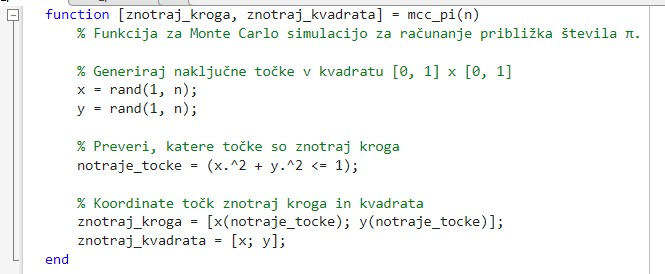
\includegraphics[width=0.8\textwidth]{mcc_pi.m.jpg}
  \end{figure}
\end{frame}

\begin{frame}{Programska datoteka}
Programska datoteka je običajno krovna datoteka, ki definira začetne vrednosti
in kliče funkcije potrebne za rešitev problema. Ustvarite programsko datoteko
\texttt{mcc\_pi.m}.
   \begin{figure}
    \centering
    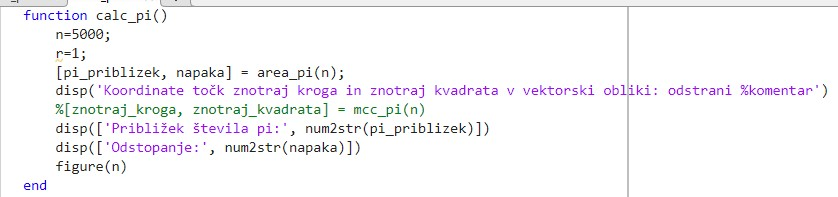
\includegraphics[width=0.9\textwidth]{calc_pi.m.jpg}
    \caption{Prvi del kode}
  \end{figure}
\end{frame}

\begin{frame}{Koordinate naključnih točk}
Funkcijo smo zakomentirali, saj nam vrne zelo dolg output. Fotografija spodaj prikazuje koordinate le nekaj naključnh točk. Opazimo, da so vse pozitivno predznačene, saj smo se pri računanju približka $\pi$ omejili na prvi kvadrant.
\begin{figure}
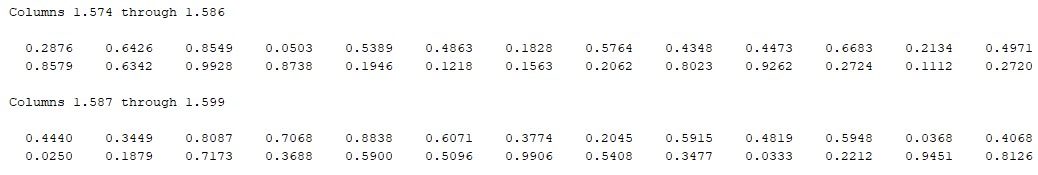
\includegraphics[width=\linewidth]{koordinate točk.jpg}
\end{figure}
\end{frame}

\section{Vizualizacija}
\begin{frame}{Vizualizacija rezultatov}
    Na prejšnji strani smo prikazali koordinate točk, ki smo jih naključno generirali z ukazom \texttt{rand}. Kot rezultat dobimo še našo ocenjeno vrednost števila $\pi$ in napako pri računanju.  S spreminjanjem števila naključnih točk $n$ ugotovimo, da je z večjim številom točk tudi rezultat bolj točen. Spodaj prikazani približek je generiran na podlagi 5000 točk.  
\begin{figure}
  \begin{minipage}{0.5\textwidth}
    \centering
    \includegraphics[width=\linewidth]{približek in napaka.jpg}
  \end{minipage}\hfill
  \pause
  \begin{minipage}{0.45\textwidth}
    \centering
    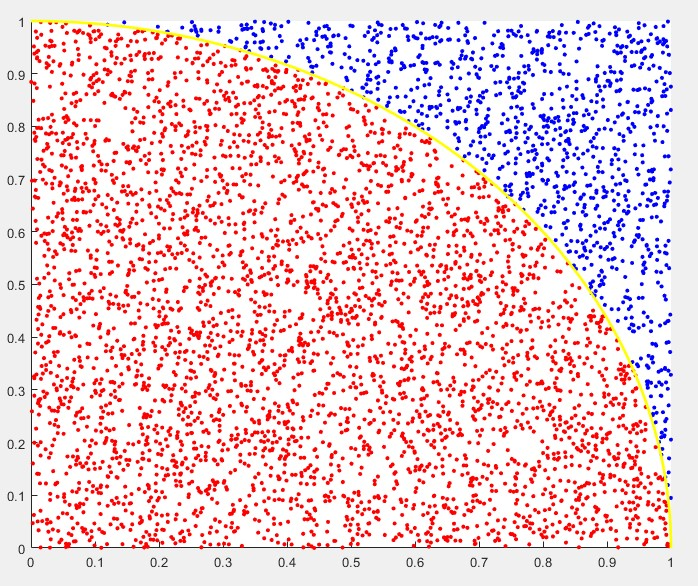
\includegraphics[width=\linewidth]{figure1.jpg}
  \end{minipage}
\end{figure}

\end{frame}

\end{document}